\documentclass[final]{beamer}

\usetheme{RJH}
\usepackage[utf8]{inputenc}
\usepackage[frenchb]{babel}
\usepackage[orientation=landscape,size=a2,scale=1.2]{beamerposter}
\usepackage[absolute,overlay]{textpos}
\usepackage{url}
\usepackage{auto-pst-pdf}
\usepackage{pst-plot}
\usepackage{graphicx}
\usepackage{color}
\usepackage{hyperref}
\usepackage{amsmath}
\usepackage{amssymb}
\usepackage{pifont}
\newcommand{\cmark}{\ding{51}}%
\newcommand{\xmark}{\ding{55}}%
\usepackage[labelformat=empty]{caption}
\usepackage{framed}

\setlength{\TPHorizModule}{\paperwidth}
\setlength{\TPVertModule}{\paperheight}

\newcommand{\qedwhite}{\hfill \ensuremath{\Box}}

\definecolor{lightgreen}{rgb}{0.094,0.737,0.611}
\definecolor{lightblue}{rgb}{0.137,0.513,0.768}
\definecolor{lightred}{rgb}{0.874,0.180,0.105}
\definecolor{gray}{rgb}{0.4,0.4,0.4}
\definecolor{lightgray}{rgb}{0.8,0.8,0.8}
\definecolor{shadecolor}{rgb}{0.9,0.9,0.9}

\title{Understanding variables importances in forests of randomized trees {\it [Sun88]}}
\author{Gilles Louppe, Louis Wehenkel, Antonio Sutera and Pierre Geurts\\[1.5ex]
{\tiny
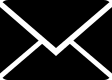
\includegraphics[scale=0.16]{images/mail.png}~\url{g.louppe@ulg.ac.be}
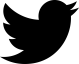
\includegraphics[scale=0.6]{images/twitter.png}~\href{https://twitter.com/glouppe}{@glouppe}

\includegraphics[scale=0.18]{images/github.png}~\url{https://github.com/glouppe/paper-variable-importances}
}}

\footer{} %\tiny \textbf{Contact}: \url{g.louppe@ulg.ac.be} $\cdot$ \href{https://twitter.com/glouppe}{@glouppe} \textbf{Code}: \url{https://github.com/glouppe/paper-variable-importances}}
\date{}

\begin{document}
\begin{frame}{}


%% Column 1 ==================================================================

\begin{textblock}{0.32}(0.01,0.14)

%% Abstract ------------------------------------------------------------------

\begin{block}{Abstract \phantom{p}}

Despite growing interest and practical use in various scientific areas, \textbf{variable
importances derived from tree-based ensemble methods are not well understood
from a theoretical point of view}. In this work we characterize the Mean Decrease
Impurity (MDI) variable importances as measured by an ensemble of totally
randomized trees in asymptotic sample and ensemble size conditions. \textbf{We derive a
three-level decomposition of the  information jointly provided by all input
variables about the output in terms of
\begin{itemize}
\item[] {\color{lightgreen}i) the MDI importance of each input variable,}
\item[] {\color{lightblue}ii) the degree of interaction of an input variable with the other input variables,}
\item[] {\color{lightred}iii) the different interaction terms of a given degree.}
\end{itemize}}
We then
show that this MDI importance of a variable is equal to zero if and only if the
variable is irrelevant and that the MDI importance of a relevant variable is
invariant with respect to the removal or the addition of irrelevant variables.
We illustrate these properties on a simple example and discuss how they may
change in the case of  non-totally randomized trees such as Random Forests and
Extra-Trees.

\end{block}

\vspace{0.5cm}
\begin{block}{Variable importances in trees \phantom{p}}

\textbf{Notations.} Let assume a set $V = \{X_1, ..., X_p\}$ of categorical input variables and a categorical output variable $Y$. Given a training sample ${\cal L}$ of $N$ joint observations of $X_1, ..., X_p, Y$ drawn from $P(X_1, ..., X_p, Y)$,
let us define for any internal node $t$ of a decision tree built from ${\cal L}$:
\begin{itemize}
\item[-] The number of training samples in $t$ as $N_t$;
\item[-] The proportion of training samples in $t$ as $p(t) = \frac{N_t}{N}$;
\item[-] The impurity of node $t$ as $i(t) = H(Y|t)$ (i.e., the Shannon entropy);
\item[-] The impurity decrease at node $t$ as $\Delta i(t) = i(t) - \frac{N_{t_L}}{N_t} i(t_L) - \frac{N_{t_R}}{N_t} i(t_R)$.
\end{itemize}

\begin{center}

\scalebox{1.0}{
    \begin{pspicture}(14,11)
    % Grid
    %\psgrid[subgriddiv=1,griddots=10,gridlabels=7pt]
    % Calcul
    \rput[l](9,9.5){\color{gray}{$i(t) = 0.97$}}
    \rput[l](9,8.5){\color{gray}{$i(t_L) = 0.65$}}
    \rput[l](9,7.5){\color{gray}{$i(t_R) = 0.81$}}
    \rput[l](9,6.5){\color{gray}{$\Delta i(t) = i(t) - \frac{12}{20} i(t_L) - \frac{8}{20} i(t_R)$}}
    \rput[l](10.55,5.5){\color{gray}{$= 0.25$}}
    % Parent node
        % Arrows
        \psline[linewidth=2pt,linecolor=lightblue]{->}(4.5,10.5)(5,10)
        \psline[linewidth=2pt,linecolor=blue]{->}(5,9)(3,7)
        \psline[linewidth=2pt,linecolor=blue]{->}(5,9)(7,7)
        % Node
        \pscircle[fillstyle=solid,fillcolor=white,linewidth=2pt,linecolor=blue](5,9){1}
        % Samples
        \psframe[fillstyle=solid,fillcolor=red,linecolor=red](4.3,9.35)(4.5,9.55)
        \psframe[fillstyle=solid,fillcolor=lightblue,linecolor=lightblue](4.6,9.35)(4.8,9.55)
        \psframe[fillstyle=solid,fillcolor=lightblue,linecolor=lightblue](4.9,9.35)(5.1,9.55)
        \psframe[fillstyle=solid,fillcolor=lightblue,linecolor=lightblue](5.2,9.35)(5.4,9.55)
        \psframe[fillstyle=solid,fillcolor=lightblue,linecolor=lightblue](5.5,9.35)(5.7,9.55)
        \psframe[fillstyle=solid,fillcolor=lightblue,linecolor=lightblue](4.3,9.05)(4.5,9.25)
        \psframe[fillstyle=solid,fillcolor=red,linecolor=red](4.6,9.05)(4.8,9.25)
        \psframe[fillstyle=solid,fillcolor=red,linecolor=red](4.9,9.05)(5.1,9.25)
        \psframe[fillstyle=solid,fillcolor=lightblue,linecolor=lightblue](5.2,9.05)(5.4,9.25)
        \psframe[fillstyle=solid,fillcolor=lightblue,linecolor=lightblue](5.5,9.05)(5.7,9.25)
        \psframe[fillstyle=solid,fillcolor=lightblue,linecolor=lightblue](4.3,8.75)(4.5,8.95)
        \psframe[fillstyle=solid,fillcolor=red,linecolor=red](4.6,8.75)(4.8,8.95)
        \psframe[fillstyle=solid,fillcolor=lightblue,linecolor=lightblue](4.9,8.75)(5.1,8.95)
        \psframe[fillstyle=solid,fillcolor=lightblue,linecolor=lightblue](5.2,8.75)(5.4,8.95)
        \psframe[fillstyle=solid,fillcolor=red,linecolor=red](5.5,8.75)(5.7,8.95)
        \psframe[fillstyle=solid,fillcolor=lightblue,linecolor=lightblue](4.3,8.45)(4.5,8.65)
        \psframe[fillstyle=solid,fillcolor=lightblue,linecolor=lightblue](4.6,8.45)(4.8,8.65)
        \psframe[fillstyle=solid,fillcolor=red,linecolor=red](4.9,8.45)(5.1,8.65)
        \psframe[fillstyle=solid,fillcolor=red,linecolor=red](5.2,8.45)(5.4,8.65)
        \psframe[fillstyle=solid,fillcolor=red,linecolor=red](5.5,8.45)(5.7,8.65)
        % Text
        \rput(6,10){$t$}
    % Left node
        % Arrows
        %\psline[linewidth=2pt,linecolor=gray](3,6)(2,5)
        %\psline[linewidth=2pt,linecolor=gray](3,6)(4,5)
        % Node
        \pscircle[fillstyle=solid,fillcolor=white,linewidth=2pt,linecolor=blue](3,6){1}
        % Samples
        \psframe[fillstyle=solid,fillcolor=lightblue,linecolor=lightblue](2.3,6.35)(2.5,6.55)
        \psframe[fillstyle=solid,fillcolor=lightblue,linecolor=lightblue](2.6,6.35)(2.8,6.55)
        \psframe[fillstyle=solid,fillcolor=lightblue,linecolor=lightblue](2.9,6.35)(3.1,6.55)
        \psframe[fillstyle=solid,fillcolor=lightblue,linecolor=lightblue](3.2,6.35)(3.4,6.55)
        \psframe[fillstyle=solid,fillcolor=lightblue,linecolor=lightblue](3.5,6.35)(3.7,6.55)
        \psframe[fillstyle=solid,fillcolor=lightblue,linecolor=lightblue](2.3,6.05)(2.5,6.25)
        \psframe[fillstyle=solid,fillcolor=lightblue,linecolor=lightblue](2.6,6.05)(2.8,6.25)
        \psframe[fillstyle=solid,fillcolor=red,linecolor=red](2.9,6.05)(3.1,6.25)
        \psframe[fillstyle=solid,fillcolor=lightblue,linecolor=lightblue](3.2,6.05)(3.4,6.25)
        \psframe[fillstyle=solid,fillcolor=lightblue,linecolor=lightblue](3.5,6.05)(3.7,6.25)
        \psframe[fillstyle=solid,fillcolor=lightblue,linecolor=lightblue](2.3,5.75)(2.5,5.95)
        \psframe[fillstyle=solid,fillcolor=red,linecolor=red](2.6,5.75)(2.8,5.95)
        % Text
        \rput(4,7){$t_L$}
        \rput(2.5,8){$X_m = 0$}
    % Right node
        % Arrows
        %\psline[linewidth=2pt,linecolor=gray](7,6)(6,5)
        %\psline[linewidth=2pt,linecolor=gray](7,6)(8,5)
        % Node
        \pscircle[fillstyle=solid,fillcolor=white,linewidth=2pt,linecolor=blue](7,6){1}
        % Samples
        \psframe[fillstyle=solid,fillcolor=red,linecolor=red](6.3,6.35)(6.5,6.55)
        \psframe[fillstyle=solid,fillcolor=red,linecolor=red](6.6,6.35)(6.8,6.55)
        \psframe[fillstyle=solid,fillcolor=lightblue,linecolor=lightblue](6.9,6.35)(7.1,6.55)
        \psframe[fillstyle=solid,fillcolor=red,linecolor=red](7.2,6.35)(7.4,6.55)
        \psframe[fillstyle=solid,fillcolor=lightblue,linecolor=lightblue](7.5,6.35)(7.7,6.55)
        \psframe[fillstyle=solid,fillcolor=red,linecolor=red](6.3,6.05)(6.5,6.25)
        \psframe[fillstyle=solid,fillcolor=red,linecolor=red](6.6,6.05)(6.8,6.25)
        \psframe[fillstyle=solid,fillcolor=red,linecolor=red](6.9,6.05)(7.1,6.25)
        % Text
        \rput(8,7){$t_R$}
        \rput(7.5,8){$X_m = 1$}
    \end{pspicture}
}
\end{center}

\textbf{Definition.} In an ensemble of decision trees, the \textit{Mean
Decrease Impurity} (MDI) importance of an input variable $X_m$ is the
sum of the weighted impurity decreases $p(t)\Delta i(t)$, for all nodes $t$
where $X_m$ is used, averaged over all $N_T$ trees in the ensemble:
\begin{align*}\label{eq:mdi}
Imp(X_m) &= \frac{1}{N_T} \sum_{T} \sum_{t \in T:v(s_t) = X_m} p(t) \Delta i(t) &&\text{(1)}
\end{align*}

\vspace{0.3cm}

\textbf{Definition.} A \textit{fully developped  totally randomized tree is a decision tree} in which each node $t$ is
partitioned using a variable $X_i$ picked uniformly at random (among those not
yet used at the parent nodes) into $|{\cal
X}_i|$ sub-trees (i.e., one for each possible value of ${\cal X}_i$) and where
the recursive construction halts when all $p$ variables have been
used along the current branch.

\end{block}

\end{textblock}



%% Column 2 ==================================================================

\begin{textblock}{0.32}(0.34,0.14)

\begin{block}{Theoretical results \phantom{p}}

{\color{green} \cmark} Thm. 1 and 2: \textbf{Variable importances provide a three-level decomposition
of the information jointly provided by all the input variables about the output}, accounting for all interaction terms in a fair and exhaustive way.\\
{\color{green} \cmark} Thm. 3 and 5: \textbf{Variable importances depend only on the relevant
variables.}

\begin{shaded}
\textbf{Theorem 1.}
\textit{The MDI importance of $X_m \in V$ for $Y$ as computed
with an   infinite ensemble of fully developed totally randomized trees and an
infinitely large training set is:}
  \begin{align*}
  Imp(X_m)&=\underbrace{\sum_{k=0}^{p-1} \frac{1}{C_p^k} \frac{1}{p-k}}_{{\color{lightblue} \substack{\text{ii) Decomposition along}\\
                                                                                                     \text{the degrees $k$ of interaction}\\
                                                                                                     \text{with the other variables}}}}
           \underbrace{\sum_{B \in {\cal P}_k(V^{-m})} I(X_m;Y|B)}_{{\color{lightred} \substack{\text{iii) Decomposition along all}\\
                                                                                                \text{interaction terms $B$}\\
                                                                                                \text{of a given degree $k$}}}}, &&\text{(2)}
  \end{align*}
\textit{\noindent where $V^{-m}$ denotes the subset $V \setminus \{X_m\}$, ${\cal
P}_k(V^{-m})$ is the set of subsets of  $V^{-m}$ of cardinality $k$, and
$I(X_m;Y|B)$ is the conditional mutual information of $X_{m}$ and $Y$ given the
variables in $B$.}
\end{shaded}

Proof. (\textit{sketch})

\begin{center}
\scalebox{1.0}{
    \begin{pspicture}(15,10)
    % Grid
    %\psgrid[subgriddiv=1,griddots=10,gridlabels=7pt]
    % Tree
        % Level 0
        \psline[linewidth=2pt,linecolor=lightgray]{->}(5,9.5)(3,8.5)
        \psline[linewidth=2pt,linecolor=lightblue]{->}(5,9.5)(7,8.5)
        \pscircle[fillstyle=solid,fillcolor=white,linewidth=2pt,linecolor=lightblue](5,9.5){0.5}
        % Level 1
        \psline[linewidth=2pt,linecolor=lightgray]{->}(3,8)(2,6.5)
        \psline[linewidth=2pt,linecolor=lightgray]{->}(3,8)(4,6.5)
        \pscircle[fillstyle=solid,fillcolor=white,linewidth=2pt,linecolor=lightgray](3,8){0.5}
        \psline[linewidth=2pt,linecolor=lightblue]{->}(7,8)(6,6.5)
        \psline[linewidth=2pt,linecolor=lightgray]{->}(7,8)(8,6.5)
        \pscircle[fillstyle=solid,fillcolor=white,linewidth=2pt,linecolor=lightblue](7,8){0.5}
        % Level 2
        \psline[linewidth=2pt,linecolor=lightgray]{->}(2,6)(1.5,4.5)
        \psline[linewidth=2pt,linecolor=lightgray]{->}(2,6)(2.5,4.5)
        \pscircle[fillstyle=solid,fillcolor=white,linewidth=2pt,linecolor=lightgray](2,6){0.5}
        \psline[linewidth=2pt,linecolor=lightgray]{->}(4,6)(3.5,4.5)
        \psline[linewidth=2pt,linecolor=lightgray]{->}(4,6)(4.5,4.5)
        \pscircle[fillstyle=solid,fillcolor=white,linewidth=2pt,linecolor=lightgray](4,6){0.5}
        \psline[linewidth=2pt,linecolor=blue]{->}(6,6)(5.5,4.5)
        \psline[linewidth=2pt,linecolor=blue]{->}(6,6)(6.5,4.5)
        \pscircle[fillstyle=solid,fillcolor=white,linewidth=2pt,linecolor=blue](6,6){0.5}
        \psline[linewidth=2pt,linecolor=lightgray]{->}(8,6)(7.5,4.5)
        \psline[linewidth=2pt,linecolor=lightgray]{->}(8,6)(8.5,4.5)
        \pscircle[fillstyle=solid,fillcolor=white,linewidth=2pt,linecolor=lightgray](8,6){0.5}
    % Labels
    \rput(7,9.25){$X_{i_1}=1$}
    \rput(5.25,7.25){$X_{i_2}=0$}
    \rput(6.5,6.5){$t$}
    \rput(4.5,5.25){$X_{m}=0$}
    \rput(7.5,5.25){$X_{m}=1$}
    % Side text
    \rput[l](11,9){$\frac{1}{C_p^k}$ is the probability of}
    \rput[l](11,8.25){the branch $B=\{X_{i_1}, X_{i_2}\}$}
    \rput[l](11,7){$\frac{1}{p-k}$ is the probability of}
    \rput[l](11,6.25){drawing $X_m$ given $B$}
    \end{pspicture}
}
\end{center}

(i) Using the Shannon entropy, $\Delta i(t) = I(X_m; Y|t)$ ;\\
(ii) As $N \to \infty$, $p(t)  \to p(B=b)$ and $I(X_m;Y|t) \to I(X_m;Y|B=b)$, where $B$ is the subset of $k$ variables in the branch leading to $t$ and $b$ the vector of values of these variables ;\\
(iii) As $N_T \to \infty$, branches $B=b$ of size $k$ all appear with equal probability $\frac{1}{C_p^k}$ and $X_m$ is tested at the end of $\frac{1}{p-k}$ of them.

$\Rightarrow$ Equation~(1) transforms into Equation~(2). \qedwhite

\vspace{0.3cm}

\begin{shaded}
\textbf{Theorem 2.}
\textit{For any ensemble of fully developed trees in asymptotic learning sample size
conditions, we have that}
\begin{align*}
\underbrace{\sum_{m=1}^{p}Imp(X_m)}_{{\color{lightgreen} \substack{\text{i) Decomposition in terms of}\\
                                                                   \text{the MDI importance of}\\
                                                                   \text{each input variable}}}} &=
\underbrace{I(X_{1}, \ldots, X_{p} ; Y)}_{\substack{\text{Information jointly provided}\\
                                                    \text{by all input variables}\\
                                                    \text{about the output}}}&&\text{(3)}
\end{align*}

\vspace{0.3cm}

\textbf{Theorem 3.}
\textit{$X_i \in V$ is irrelevant to $Y$ with respect to $V$ if and only if  its
infinite sample size importance as computed with an infinite ensemble of fully
developed totally randomized trees built on $V$ for $Y$ is 0.}

\vspace{0.3cm}

\textbf{Theorem 5.}
\textit{Let $V_R \subseteq V$ be the subset of all variables in $V$ that are relevant to $Y$ with
respect to $V$. The infinite sample size importance of any variable $X_m \in
V_R$ as computed with an infinite ensemble of fully developed totally randomized
trees built on $V_R$ for $Y$ is the same as its importance computed in the same conditions by using all variables in $V$.}
\end{shaded}

\end{block}

\end{textblock}


%% Column 3 ==================================================================

\begin{textblock}{0.32}(0.67,0.14)

\begin{block}{Non-totally randomized trees \phantom{p}}

{\color{red} \xmark} Because of masking effects due to the non-totally random
choices of split variables, \textbf{Theorems 1, 3 and 5 do not apply for Random Forests}
and variants. Increasing $K$ (aka. \textit{mtry} or \textit{max\_features} -- the number of variables drawn
to maximize $\Delta i$) makes importance scores diverge from a fair and
exhaustive exploration of all interaction terms.

\end{block}

\begin{block}{Illustration \phantom{p}}

\textbf{Task.} Let us consider a 7-segment indicator, as shown in Fig (a), displaying numerals
using lights in on-off combinations. Let $Y$ be a random variable taking its value in $\{0, 1, ..., 9\}$
and let $X_1, ..., X_7$ be binary variables corresponding to the light segments. We illustrate
variable importances as computed with totally randomized trees built
from training samples drawn from $P(X_1, ..., X_7, Y)$.

\begin{minipage}[b]{\textwidth}
  \begin{minipage}[t]{0.3\textwidth}
    \centering
    \begin{pspicture}(0,0)(2.0,4.0)
        \usefont{T1}{ptm}{m}{n}
        \psline[linewidth=0.02cm](0.0,0.0)(0.0,0.7)
        \psline[linewidth=0.02cm](0.0,0.0)(0.7,0.0)
        \psline[linewidth=0.02cm](2.0,0.0)(2.0,0.7)
        \psline[linewidth=0.02cm](2.0,0.0)(1.3,0.0)
        \psline[linewidth=0.02cm](0.0,2.0)(0.0,1.3)
        \psline[linewidth=0.02cm](0.0,2.0)(0.7,2.0)
        \psline[linewidth=0.02cm](2.0,2.0)(2.0,1.3)
        \psline[linewidth=0.02cm](2.0,2.0)(1.3,2.0)
        \psline[linewidth=0.02cm](0.0,2.0)(0.0,2.7)
        \psline[linewidth=0.02cm](2.0,2.0)(2.0,2.7)
        \psline[linewidth=0.02cm](0.0,4.0)(0.0,3.3)
        \psline[linewidth=0.02cm](0.0,4.0)(0.7,4.0)
        \psline[linewidth=0.02cm](2.0,4.0)(2.0,3.3)
        \psline[linewidth=0.02cm](2.0,4.0)(1.3,4.0)
        \rput(1.0,4.0){$X_1$}
        \rput(0.0,3.0){$X_2$}
        \rput(2.0,3.0){$X_3$}
        \rput(1.0,2.0){$X_4$}
        \rput(0.0,1.0){$X_5$}
        \rput(2.0,1.0){$X_6$}
        \rput(1.0,0.0){$X_7$}
    \end{pspicture}
    \captionof{figure}{\tiny (a)}
    \label{fig:digits}
  \end{minipage}
  \hfill
  \begin{minipage}[t]{0.65\textwidth}
    \centering
    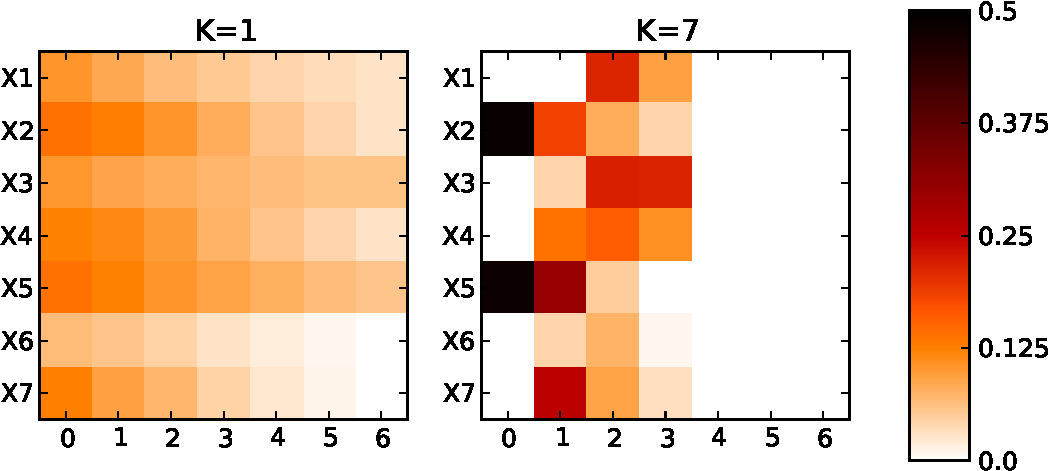
\includegraphics[scale=0.65]{images/imp-led.pdf}
    \captionof{table}{\tiny (b)}
    \label{table:digits}
  \end{minipage}
\end{minipage}

Fig (b) illustrates the decomposition of variable importances along the
degrees $k$ of interactions of one variable with the other ones. At $K=1$, all
$I(X_m;Y|B)$ are accounted for in the total importance, while at $K=7$ only
some of them are taken into account due to masking effects.


\begin{table}
    \scalebox{0.8}{
    \begin{tabular}{ c | c c c c c c c c }
    \hline
        & Thm.1 & $K=1$ & $K=2$ & $K=3$ & $K=4$ & $K=5$ & $K=6$ & $K=7$ \\
    \hline
    $X_1$ & 0.412 & 0.414 & 0.362 & 0.327 & 0.309 & 0.304 & 0.305 & 0.306\\
    $X_2$ & 0.581 & 0.583 & 0.663 & 0.715 & 0.757 & 0.787 & 0.801 & 0.799\\
    $X_3$ & 0.531 & 0.532 & 0.512 & 0.496 & 0.489 & 0.483 & 0.475 & 0.475\\
    $X_4$ & 0.542 & 0.543 & 0.525 & 0.484 & 0.445 & 0.414 & 0.409 & 0.412\\
    $X_5$ & 0.656 & 0.658 & 0.731 & 0.778 & 0.810 & 0.827 & 0.831 & 0.835\\
    $X_6$ & 0.225 & 0.221 & 0.140 & 0.126 & 0.122 & 0.122 & 0.121 & 0.120\\
    $X_7$ & 0.372 & 0.368 & 0.385 & 0.392 & 0.387 & 0.382 & 0.375 & 0.372\\
    \hline
    $\sum$& 3.321 & 3.321 & 3.321 & 3.321 & 3.321 & 3.321 & 3.321 & 3.321\\
    \hline
    \end{tabular}}
\end{table}

Variable importances at $K=1$ follow their theoretical values,
as predicted by Theorem~1. However, as $K$ increases,  importances diverge due
to masking effects. In accordance with Theorem~2, their sum is also always
equal to $I(X_{1}, \ldots, X_{7}; Y) = H(Y) = \log_{2}(10)= 3.321$ since inputs
allow to perfectly predict the output


\end{block}

\vspace{0.5cm}
\begin{block}{Conclusions \phantom{p}}

{\color{green} \cmark} First step towards understanding variable importances, as computed with a forest of totally randomized trees.

{\color{green} \cmark} Variable importances offer a three-level decomposition of the information provided by the inputs about the output.

{\color{green} \cmark} MDI importances exhibit desirable properties for assessing the relevance of a variable:
\begin{itemize}
\item[-] it accounts for all interaction terms, in a fair and exhaustive way;
\item[-] it is null if and only if the variable is irrelevant;
\item[-] it depends only on the relevant variables;
\end{itemize}

{\color{blue} ?} Fully formalize variable importances of actual Random Forests and variants.

{\color{blue} ?} Characterize the distribution of variable importances in a finite setting.


\end{block}

\end{textblock}




\end{frame}
\end{document}
